\documentclass[runningheads]{llncs}

\usepackage[T1]{fontenc}
\usepackage{graphicx}
\usepackage{xparse} % interval
\usepackage{listings} % code

%%------------------------------------------------
%%------------------------------------------------

\begin{document}
\title{Computer Networks Project: \\ Romanian Railways}

\author{P. Braha\inst{1}\orcidID{0009-0001-3636-2455}}
\authorrunning{P. Braha}
\institute{Alexandru Ioan Cuza University, Iasi IS 700221, Romania
\email{petrubraha@gmail.com}\\
\url{https://github.com/petru-braha}}

\maketitle

\begin{abstract} This work contains an overview of the client-server paradigm offering, to the public transport companies, a concrete (and open-source) informational system connected with potential clients. This system notifies consumers about the traveling schedule for the current day, the available means of transport (e.g., trains) associated with their time and location, and other related knowledge such as status of departure/arrival and vehicle identification. Any user can report late arrivals, but in a controlled manner such that the misleading records are checked and ignored, if necessary. The application achieves great communication speed with the customers, minimizing the risk of damage to the data quality. Currently, the server application is continuously running and ready to serve queries. One particular limitation regarding security is the single point of failure. With some financial investments, the code base could be generalized to integrate multiple server ends. This paper represents an implementation reference for network programming and administration, completely reviewing my repository.

\keywords{Server \and Client \and Application level \and Transport level \and I/O multiplexing \and TCP \and UDP \and Thread \and Socket }
\end{abstract}

%%------------------------------------------------
%%------------------------------------------------

\section{Introduction}

"Romanian Railways" is a multi-paradigm project that involves compiling two programs: one for the server and the other for the client(s). It is in a professional working state, with one server instance running indefinitely at $10.100.0.30:2970$. The maximum capacity of connected users is 1024 per server instance. The server holds traveling schedules for the current date, and clients can query routes from a specific location or time and report delays.

This document continues to explain some requirements and the logic behind the code. The following section will explore a short list of the adopted technologies. Choosing the right tools will determine the overall quality of the apps. In the third chapter, you may find the structure of the server application and a illustration of the routines executed. Following this, additional details, experiments, and observations are analyzed. The advantages and roles of the implementation decisions are discussed. This part opens up the API definitions at the application level. Last but not least, the conclusions will summarize my project and propose some scenarios where the "RR-application" could be helpful.

\subsection{Motivation}

The entire repository is a matter of personal interest for the "Computer Networks" course. Officially, it is known as laboratory homework, but the main goal is far higher: contributing to practical life. When designing this project, I was encouraged to provide an optimal and creative implementation.

\section{Applied Technologies}

In the development, three main core objectives were followed: speed, correctness, and security. Therefore, the C programming language was elected because:
\begin{itemize}
  \item it is one of the fastest compiled languages;
  \item it supplies network management resources, such as threads and sockets;
  \item it delivers simple syntax, yet highly customizable flags and options (important for the non-blocking calls);
  \item it has all the necessary tools to assure the objectives previously considered; a more advanced language like C++ would add an layer of unnecessary complexity.
\end{itemize}

The server application must be concurrent; otherwise, a queue of clients would be formed, and their requests would be delivered slowly. A thread-based schema benefits from multiple gains over process copies.

Messages are exchanged between customers and the server using sockets with both TCP and UDP.

%%------------------------------------------------
%%------------------------------------------------

\section{Application Structure}

The diagram of the core procedures is on the next page. Breaking down the components into POSIX's standard syntax will form a compact overview that is easy to follow.

Let us start commenting "server.c"; there are two main frames: the initialization stage and the loop. The initialization begins by creating an empty set of socket descriptors - one per customer. Then, it sets up two non-blocking sockets by linking them with the server's address. The first socket is the preliminary step of the TCP's three-way handshake (listens for connections), while the second involves UDP transmissions.

The initialization stage ends when the initial process is divided into three threads; thus, the loop starts. The root thread (the middle one) accepts new connections, while the others organize the data travel. The ioctl() function adds the non-blocking feature to the latest accepted clients' sockets. They will also be placed in the socket set initialized earlier. The following thread to be discussed (the one from the right) takes advantage of this set. The socket operations will always be non-blocking. That's why I/O multiplexing is necessary. Briefly, the communication with the clients uses TCP here. The last thread (the far left one) also has non-blocking reads and writes but with UDP datagrams.

\newpage
\begin{figure}[!h]
  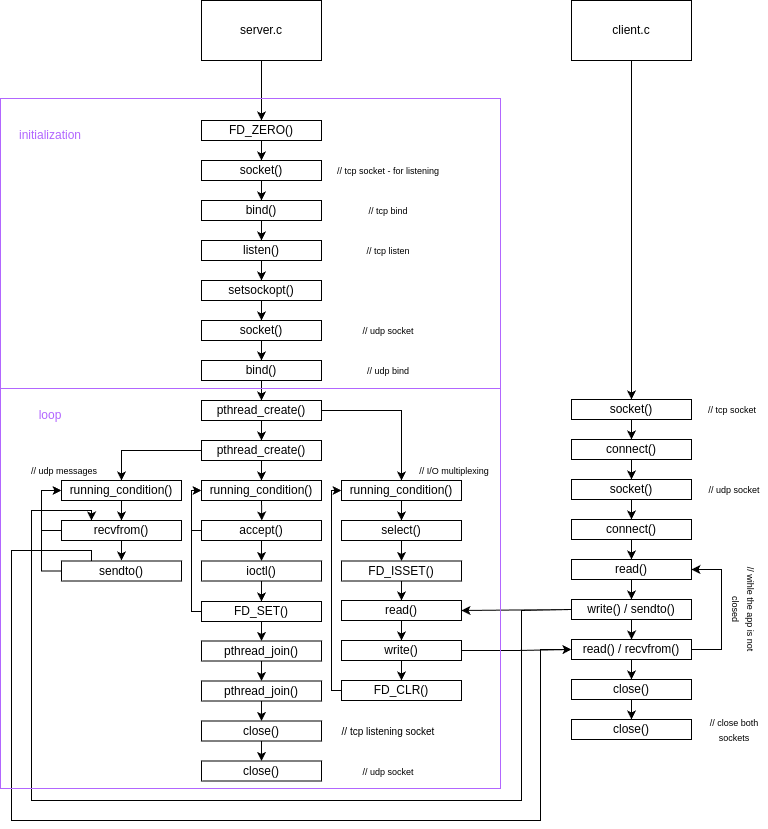
\includegraphics[width=\textwidth]{RR execution diagram.drawio.png}
  \caption{Execution illustration, made with \cite{diagram-site}} 
  \label{fig:exe}
\end{figure}

Note that running\_condition() always returns true, with one exception: an "administrative key" that stops the algorithm and closes the server. The file "include/dev/key.txt" influences the behavior of the about function. The administrator could close the server if he empties the content of this file. If no changes are registered to it, the server will continue running.

Considering the server's structure, every client needs two sockets. Depending on their request, the message is sent using either read() and write(), or sendto() and recvfrom(). The client application also runs in a loop, allowing the user to explore different updates live. Note that the client's connection-less socket is associated with connect() (more here: \cite{udp-connect}).

%%------------------------------------------------
%%------------------------------------------------

\section{Implementation Aspects}

The current code's base follows the TCP stack model but with a refined blueprint outlined in the following subsections.

\subsection{Concurrency schema}

The following list of strategies were evaluated in the latest release:
\begin{itemize}
  \item pre-forking;
  \item pre-threading;
  \item fork per client;
  \item thread per client.
\end{itemize}

Using threads over child processes is due to their "shared memory" character (please also note: \cite{fork-vs-thread}). Even if a child process is "copy on write" optimized, it is not the best choice for a long-term running server that frequently updates all of the data. 

What about the "pre-threading"? Approaching this requires fixing a specific number of threads, say $x$, which could be overwhelmed by $x + 1$ clients. This fault could be countered by adding threads for exceeding customers. Theoretically speaking, this is the obvious choice. But there is a catch: hardware. Having too many threads could slow down the computing power drastically. Knowing that the server application should be compatible with systems with a limited number of cores, this approach is not optimal. What if multiple server instances will be running in sync in the future? The constant number of threads has to adapt to machines with different components.

So, the final configuration is a hardware-portable combination of the second approach and I/O multiplexing. The server works with only three threads. Let the basic iterative TCP server be our guide for now (an example can be viewed here: \cite{course} - week 5). It has to accept connections, manage descriptors, and send data. Wouldn't it be faster to run these concurrently? The previously discussed picture precisely foreshadowed this. One thread takes care of the connections, another checks which customers are ready to be dealt with, and the last one's role is to provide a gateway for connection-less requests.

\subsection{I/O Multiplexing}

This topic further improves the speed of client-server correspondence. The select() primitive with unblocking I/O operations is considered to bring exceptional results (accordingly to \cite{non-block-select} and \cite{course} - week 7). What is better than an iterative server with I/O multiplexing? A concurrent one that uses the same principle.

\subsection{Transport protocol}

The transport layer uses a combination of TCP and UDP, and the code exploits their advantages in the appropriate situations.

The TCP protocol is used for commands that influence the server's data. Being a secure protocol, TCP provides acknowledgments for all transmitted messages. However, it implies an increased amount of time, which proposes the usage of the UDP protocol. TCP is a robust mechanism that assures the correctness of transmissions, which is mandatory for clients' reports. But in cases of straightforward queries, faster communication is preferred. If the communication fails, it can be readdressed by the consumer.

Wrong outputs were avoided. The clients must resend the same query if nothing is received at one end. If something false is received at the server's end, it can interpret and remodel the request. The only way to check if an output is correct on the customer's end is to resend the query.

Briefly, the clients use TCP to send requests to change the trains' schedule and UDP to retrieve information.

\subsection{Innovative scores}

Including an "administrative key" is a simple yet valuable contribution. Instead of manually crashing the server, an admin uses the key, running\_condition() returns false, and the server automatically shuts down, avoiding memory leaks and errors.

A unique feature is the data generation. This project allows the network administrator to either randomly generate the schedules or to provide a file with this data. By default, the server creates new routes daily, which is done using a pseudo-random number generator, Mersenne Twister. Firstly, the traveling schedule is locatated in "include/data/" (stored as xml/txt files) and then processed by the server in an actual buffer.

This mechanism is executed at maintenance time and initialization. "Maintenance" is a routine that runs once per day and updates the schedule for the current date. At 00:00 GMT+2, it is being set to close all sockets, communication channels, and threads. All the data from the previous day is then flushed and replaced by new routes. These routes are randomly generated if in the server initialization were too. Otherwise, the server looks into the file passed at initialization and checks if there are changes. The new itineraries replace everything in that unique file.

To increase transmission speed, the data's size has to be minimal. In this case, an array of routes is minimized by having each element as light as possible. A route is designed to only weight eight bytes. Why can't it be lower than that? Because it has to contain information about departures' location and time (analogous to arrivals), status, and the vehicle's id. The last two need to be separated fields, but location and time for departure/arrival are merged into only one address. So, the total traveling schedule's size is only 80 MB at maximum. A complete walkthrough of these concepts can be found in "docs/brainstorm.md".

\newpage
\section{Application protocol}

\subsection{Definitions}

In the succeeding lines the dialect used in the application protocol is described.

\begin{itemize}
  \item route = an itinerary is from point A to point B with no other points in between (A != B). In memory it is composed of an vehicle number, two location points, two time delimitations and a status field, forming a rr\_route struct.

  \item locations types: departures, arrivals. They are being recognized as integers.

  \item estimated times = initial times defined by the generated schedule
  \item confirmed times = estimated times +/- delays. A clear distinction is made between "estimated" and "confirmed". The former has an information initializing character, while the second emphasizes that the information is a subject to modifications.
    
  \item times types: confirmed departure time, estimated departure time, confirmed arrival time, estimated arrival time.
    
  \item status of a train = indicates if the current vehicle whether it has left the departure location or arrived at destination. Both will be as a boolean variable int the rr\_status struct.

  \item usht = unsigned short
  \item the time of the application is GMT+2 - Romania's time. 
  \item the trains, for more than three hours late, are considered faulted.
\end{itemize}

\subsection{API}

The following commands should be perceived from the client's point of view.

\begin{enumerate}
  \item \begin{itemize} 
    \item NAME: routes - trains departing from A to B for the current day.
    \item SYNOPSIS: struct rr\_route* routes(usht location\_departure, usht location\_arrival);
    \item DESCRIPTION: Receives as parameters the poitns A and B (the desired travel path) and iterates through the all the routes for matching location settings.
    \item RETURN VALUE: On success, routes() returns an integer - the count of searched routes - and a pointer to the schedule's data. On failure, it returns 0 and a NULL-pointer.
    \item NOTES: It follows the UDP transmission type. If one of the descriptors is invalid the function fails.
    \item ANALOGY:
      \begin{lstlisting}[language=C++]
        unsigned short IASI = 23;
        unsigned short BUCHAREST = 24;
        struct rr_route* it = routes(IASI, BUCHAREST);
        while(it){
          sendto(sd, *it, sizeof(struct rr_route));
          it++; 
        }
      \end{lstlisting}
    \vspace{0.3cm}
  \end{itemize}
   
  \item \begin{itemize}
    \item NAME: departures - trains departing from A to anywhere in the next hour.
    \item SYNOPSIS: struct rr\_route* departures(usht location\_departure);
    \item DESCRIPTION: It iterates through all the routes and checks the current time of the day, the departure location field, alongside its corresponding time. 
    \item RETURN VALUE: On success, departures() returns an integer - the count of searched routes - and a pointer to the list of the routes matching the above requirements. On failure, it returns 0 and NULL-pointer.
    \item NOTES: It follows the UDP transmission type.
    \vspace{0.3cm}
  \end{itemize}
   
  \item \begin{itemize}
    \item NAME: arrivals - trains departing from anywhere to B in the next hour.
    \item SYNOPSIS: struct rr\_route* arrivals(usht location\_arrival);
    \item DESCRIPTION: It iterates through  all the routes and checks the current time of the day, the arrival location field, alongside its corresponding time. 
    \item RETURN VALUE: On success, arrivals() returns an integer - the count of searched routes - and a pointer to the list of the routes matching the above requirements. On failure, it returns 0 and NULL-pointer.
    \item NOTES: It follows the UDP transmission type.
    \vspace{0.3cm}
  \end{itemize}
   
  \item \begin{itemize}
    \item NAME: report - sends requests to update a route's data.
    \item SYNOPSIS: bool report(usht id\_train, usht minutes);
    \item DESCRIPTION: If id\_train is smaller than the routes' count, it is indexed in the routes' array to search for the delay\_data field. If it is not already faulted, the delay time is updated it accordingly to client's request.
    \item NOTES: It follows the TCP transmission type. If the above conditions are not validated, the method returns false.
    \item ANALOGY:
      \begin{lstlisting}[language=C++]
        /* let 100 be an arrived train,
        101 a departed train not marked as arrived, 
        102 a train not marked as departed*/
        
        report(100, 5);     // fails
        report(101, 5);     // works
        report(101, 181);   // works, faulted
        report(102, 15);    // fails
      \end{lstlisting}
    \vspace{0.3cm}
  \end{itemize}
   
  \item \begin{itemize}
    \item NAME: quit - allows the consumer to close the application.
    \item SYNOPSIS: bool quit();  
    \item DESCRIPTION: This function is definite in closing the communication with the server. Once typed the application will close.
    \item NOTES: It follows the TCP transmission type. If the client's application crashes unexpectedly with no quit() call, the server is notified about the event and displays a warning in the console. The only time when it returns false is when server crashes before customer exits.
  \end{itemize}
\end{enumerate}

%%------------------------------------------------
%%------------------------------------------------

\newpage
\section{Conclusions}

For what is this project suitable for?

Clearly, its rich documentation and open-source code suit it for studying low-level C's network API. 

Since it includes a complete implementation, it could be professionally used right now in scenarios like public transport, production industries, managerial work, personal lists, etc. The design of "trains" can be extrapolated to states. Any industry whose tasks can be tracked using schedules can use this application. The only change produced is the data encoding because the system is viable and can be generalized easily.

Finally, this work concludes as a reference for the applied principles of network management. It showcases a fast, correct, and secure implementation that uses many different approaches to maximize these goals. To increase speed, a pre-threaded execution, UDP, and a hybridized TCP with I/0 multiplexing were utilized.

\begin{credits}
  \subsubsection{\ackname} This open-source project has no financial support. Improvements and updates are no longer expected.
  \subsubsection{\discintname} There are no competing interests to declare, that could be relevant to the content of this article.
\end{credits}
    

%%------------------------------------------------
%%------------------------------------------------

\begin{thebibliography}{8}

\bibitem{diagram-site} "draw.io". Diagram drawing tool. \\ \url{https://app.diagrams.net/}

\bibitem{udp-connect}
T. Gavrichenkov. "Can you bind() and connect() both ends of a UDP connection". Stack Overflow. Accessed on 29.11.2024. \\
\url{https://stackoverflow.com/questions/9741392/can-you-bind-and-connect-both-ends-of-a-udp-connection}

\bibitem{fork-vs-thread} Sysel, Martin. "A comparison of processes and threads creation". Software Engineering Perspectives in Intelligent Systems: Proceedings of 4th Computational Methods in Systems and Software 2020, Vol. 1 4. Springer International Publishing, 2020. \\ 
\doi{10.1007/978-3-030-63322-6_85}

\bibitem{course}
L. Alboaie, A. Panu. "Computer Networks" - course page. Alexandru Ioan Cuza University, 2024. \\
\url{https://edu.info.uaic.ro/computer-networks/index.php}

\bibitem{non-block-select} Stevens, W. Richard, Andrew M. Rudoff, and Bill Fenner. Unix network programming volume 1: the sockets networking API. Vol. 3. Boston: Addison-Wesley Professional, 2003.

\bibitem{ibm} "Example: Nonblocking I/O and select()". IBM's company. Accessed on 26.11.2024. \\
\url{https://www.ibm.com/docs/en/i/7.3?topic=designs-example-nonblocking-io-select}

\end{thebibliography}
\end{document}
